\section{Sistema de Cómputo}


\begin{ejercicio}\label{ej:1.Ejercicio1}
    El método de comunicación de E/S en el que la CPU está esperando hasta que la operación de E/S ha
    finalizado se conoce como:
    
    \begin{enumerate}[label=(\alph*)]
      \myitem \textbf{E/S Programada.}
      \item E/S Dirigida por Interrupciones.
      \item DMA.
      \item E/S a Distancia.
    \end{enumerate}
    
\end{ejercicio}

\begin{ejercicio}\label{ej:1.Ejercicio2}
    El método de comunicación de E/S en el que el dispositivo de E/S informa a la CPU en qué momento está 
    preparado el dispositivo para la transferencia de datos se conoce como:
    
    \begin{enumerate}[label=(\alph*)]
      
      \item E/S Programada.
      \myitem \textbf{E/S Dirigida por interrupciones.}
      \item DMA.
      \item E/S a Distancia.
    \end{enumerate}
    
\end{ejercicio}

\begin{ejercicio}\label{ej:1.Ejercicio3}
    Cuál de las siguientes afirmaciones es correcta:
    
    \begin{enumerate}[label=(\alph*)]
      
      \item En algunas computadoras un programa puede ejecutarse sin necesidad de cargarlo en la memoria principal.
      \myitem \textbf{Un programa, para que se ejecute, debe estar cargado en la memoria principal}
      \item Un programa, para que se ejecute, basta con que esté en el disco duro
      \item Un programa, para que se ejecute, si está en lenguaje máquina, puede estar en cualquier unidad.
    \end{enumerate}
    
\end{ejercicio}

\begin{ejercicio}\label{ej:1.Ejercicio4}
    Dado el esquema de un computador elemental según se ha descrito en el tema, el puntero de pila (SP) indica:
    
    \begin{enumerate}[label=(\alph*)]
      
      \item La dirección de memoria donde debe saltar el programa después de ejecutarse la instrucción de retorno correspondiente.
      \myitem \textbf{La dirección de memoria donde se encuentra la dirección donde debe saltar el programa después de 
      ejecutarse la instrucción de retorno correspondiente}\footnote{En realidad apunta a la dirección de memoria anterior.}.
      \item La dirección de memoria a donde se ha producido el último salto.
      \item La dirección de memoria donde se encuentra la dirección a donde se ha producido la última llamada a una subrutina.
    \end{enumerate}
    
\end{ejercicio}





% Ejercicio 5 de la relacion ---------------------------------------------
	
\begin{ejercicio}\label{ej:1.Ejercicio5}
    Sea un ordenador elemental con una arquitectura tal y como se muestra en la figura \ref{fig:Ej5_Computador}, es decir, tres registros de propósito general, registro contador de programa (PC) y registro de instrucción (IR). El registro SP (Puntero de pila) contiene la dirección 35 y la pila crece hacia posiciones menores de memoria. La memoria principal dispone de 256 palabras donde cada palabra tiene la longitud necesaria para albergar la instrucción de mayor tamaño. Describa el estado final de ejecución del procesador a partir del estado actual de la CPU mostrado en la figura \ref{fig:Ej5_Computador}. Ponga todos los valores de los registros de cada ciclo de instrucción realizado por el procesador hasta llegar a dicho estado final.
    \begin{figure}[H]
        \centering
        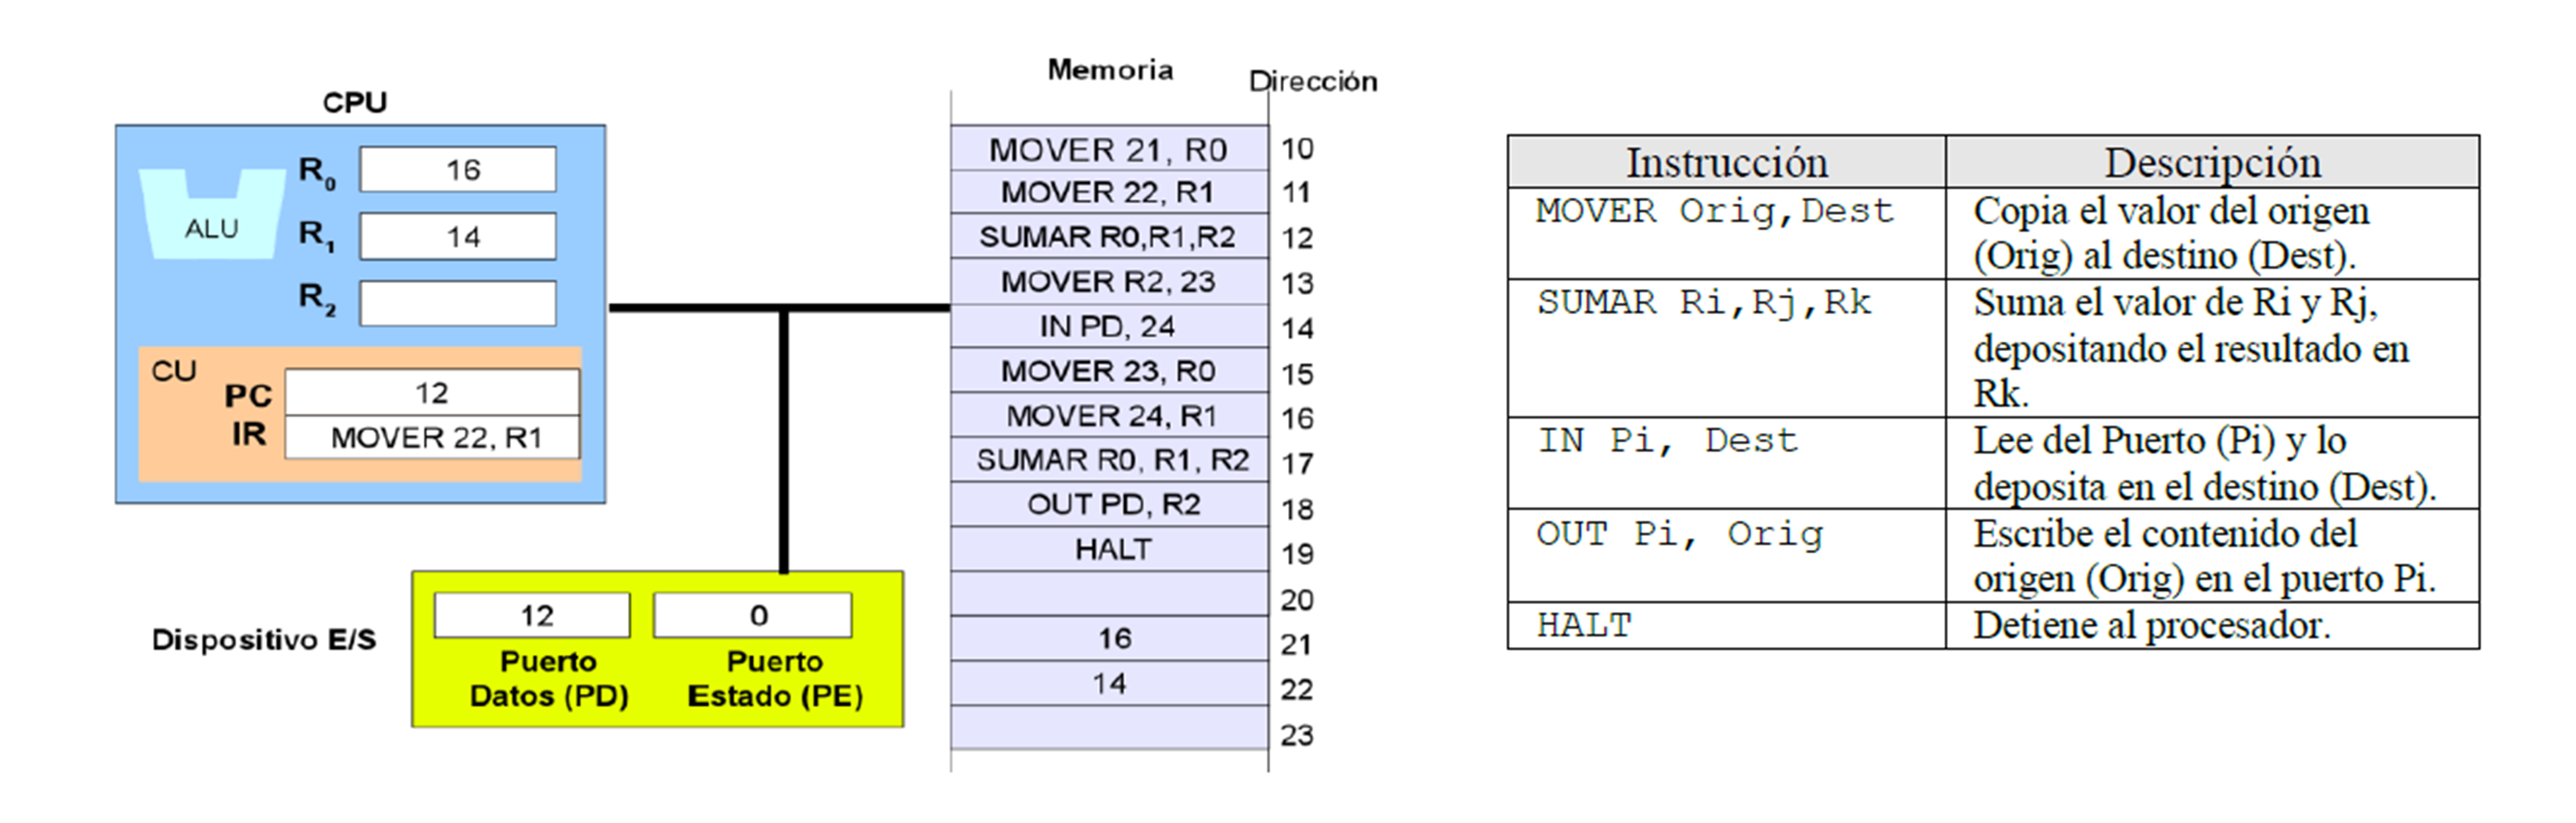
\includegraphics[width=1.1\linewidth]{Imagenes/Ej5_Compuatdor.png}
        \caption{Computador del ejercicio \ref{ej:1.Ejercicio5}}.
        \label{fig:Ej5_Computador}
    \end{figure}

    El estado del computador en cada ciclo es:
    \begin{table}[H]
        \centering
        \begin{tabular}{c|c|c|c|c|c|c|c}
            PC & IR & SP & R0 & R1 & R2 & PE & PD \\ \hline
            12 & MOVER 22, R1 & 35 & 16  & 14  &  & 0 & 12 \\
            13 & SUMAR R0,R1,R2 & 35 & 16 & 14 & 30 & 0  & 12 \\
            14 & MOVER R2,23  & 35 & 16  & 14 & 30 & 0 & 12  \\
            15 & IN PD 24 & 35 & 16  & 14 & 30 & 0 & 12  \\
            16 & MOVER 23, R0  & 35 & 30  & 14 & 30 & 0 & 12  \\
            17 & MOVER 24, R1  & 35 & 30  & 12 & 30 & 0 & 12  \\
            18 & SUMAR R0,R1,R2  & 35 & 30  & 12 & 42 & 0 & 12  \\
            19 & OUT PD, R2  & 35 & 30  & 12 & 42 & 0 & 42  \\
            20 &  HALT  & 35 & 30  & 12 & 42 & 0 & 42  \\
        \end{tabular}
        \caption{Ejecución del programa del ejercicio \ref{ej:1.Ejercicio5}}
        \label{tab:Ejercicio5}
    \end{table}
    
    \begin{table}[H]
        \centering
        \begin{tabular}{|c|c}
            Memoria & \\ \hline
            & $\vdots$ \\
            16 & 21\\
            14 & 22\\
            30 & 23\\
            12 & 24\\
            & $\vdots$ \\
        \end{tabular}
        \caption{Memoria del ejercicio \ref{ej:1.Ejercicio5}}
        \label{tab:MemEjercicio5}
    \end{table}
\end{ejercicio}

% Ejercicio 6 de la relacion ---------------------------------------------
\begin{ejercicio}
    Suponiendo que el lenguaje máquina de la arquitectura anterior dispone de 14 instrucciones distintas, muestre cuántos bits serían necesarios para codificar las instrucciones SUMAR R0,R1,R2 y MOVER 20,R0 respectivamente.\\
    
    Puesto que dispone de 14 instrucciones distintas, se necesitaran 4 bits para codificarlas. 
    \begin{itemize}
        \item \textbf{SUMAR R0, R1, R2: } Son necesarios además 2 bits para codificar cada uno de los 3 registros. Luego $4+3\cdot2 = 10$ bits
        \item \textbf{MOVER 20, R0: } Son necesarios además 2 para el registro R0. Para codificar la dirección, puesto que hay $256=2^8$ palabras de memoria principal, se necesitan 8 bits por dirección. Luego $4+2+8=14$ bits
    \end{itemize}
    
\end{ejercicio}

\begin{ejercicio}\label{Ejercicio7}
    Imagina que el procesador está ejecutando el programa de usuario del ejercicio \ref{ej:1.Ejercicio5} y en este momento al terminar de ejecutar la instrucción actual, el procesador se da cuenta de que hay una interrupción pendiente. Escribe los pasos que se dan en el sistema y por quién (software o hardware) hasta que se resuelve el tratamiento de la interrupción y el programa finaliza, sabiendo que la rutina de tratamiento de la interrupción comienza en la dirección de memoria principal 56 y termina en la dirección de memoria principal 70.\\

    \noindent En primer lugar, a nivel de hardware, se da:
    \begin{enumerate}
        \item El procesador indica el reconocimiento de la interrupción.
        \item El procesador apila PSW y el PC en la pila de control. Es decir:
            \begin{equation*}
                 M[35]=PC=12 \quad M[34-n]=PSW \quad SP=33-n
            \end{equation*}
        \item \label{Ej7:UltItem} El procesador carga un nuevo valor en el PC basado en la interrupción. En este caso, como la interrupción comienza en la dirección 56, $PC=56$.
    \end{enumerate}

    \noindent A nivel de software, se da:
    \begin{enumerate}[resume]
        \item Se salva el resto de la información de estado del proceso.
        \item Se procesa la interrupción. En este caso, se ejecutan las instrucciones desde la posición 56 a 70. Es decir, al terminar, $PC=71$.
        \item Se restaura la información de estado del proceso.
        \item Se restauran los valores de PSW y PC y se actualiza el puntero de pila. Es decir,
        \begin{equation*}
            PSW=M[34-n] \quad PC=M[35]=12 \quad SP=35
        \end{equation*}
    \end{enumerate}
\end{ejercicio}

\begin{ejercicio}
    Basándonos en el ejercicio \ref{Ejercicio7}, ¿hay diferencias si en vez de producirse una interrupción se ha producido una excepción? Indique cuales.\\

    Sí, hay diferencias. En primer lugar, las excepciones son un evento síncrono, mientras que las interrupciones son asíncronas. El procesador aquí se ha dado cuenta al finalizar la ejecución de que había una interrupción pendiente, mientras que en el caso de una excepción se ejecuta directamente. Además, por norma general, una excepción conlleva un posible error en el código y cómo resolverlo, mientras que las interrupciones no suelen estar asociadas a errores.
\end{ejercicio}


\begin{ejercicio}\label{ej:1.Ejercicio9}
    Sea un ordenador elemental con una arquitectura tal y como se muestra en la figura \ref{fig:Ej9_Computador}, es decir, tres registros de propósito general, registro contador de programa (PC), registro de instrucción (IR) y registro de pila (SP). La memoria principal dispone de 512 palabras donde cada palabra tiene la longitud necesaria para albergar la instrucción de mayor tamaño. Describa el estado final de ejecución del procesador a partir del estado actual de la CPU mostrado en la figura y tras la ejecución del programa (nótese que la instrucción de la dirección 10 ya se ha ejecutado).
    \begin{figure}[H]
        \centering
        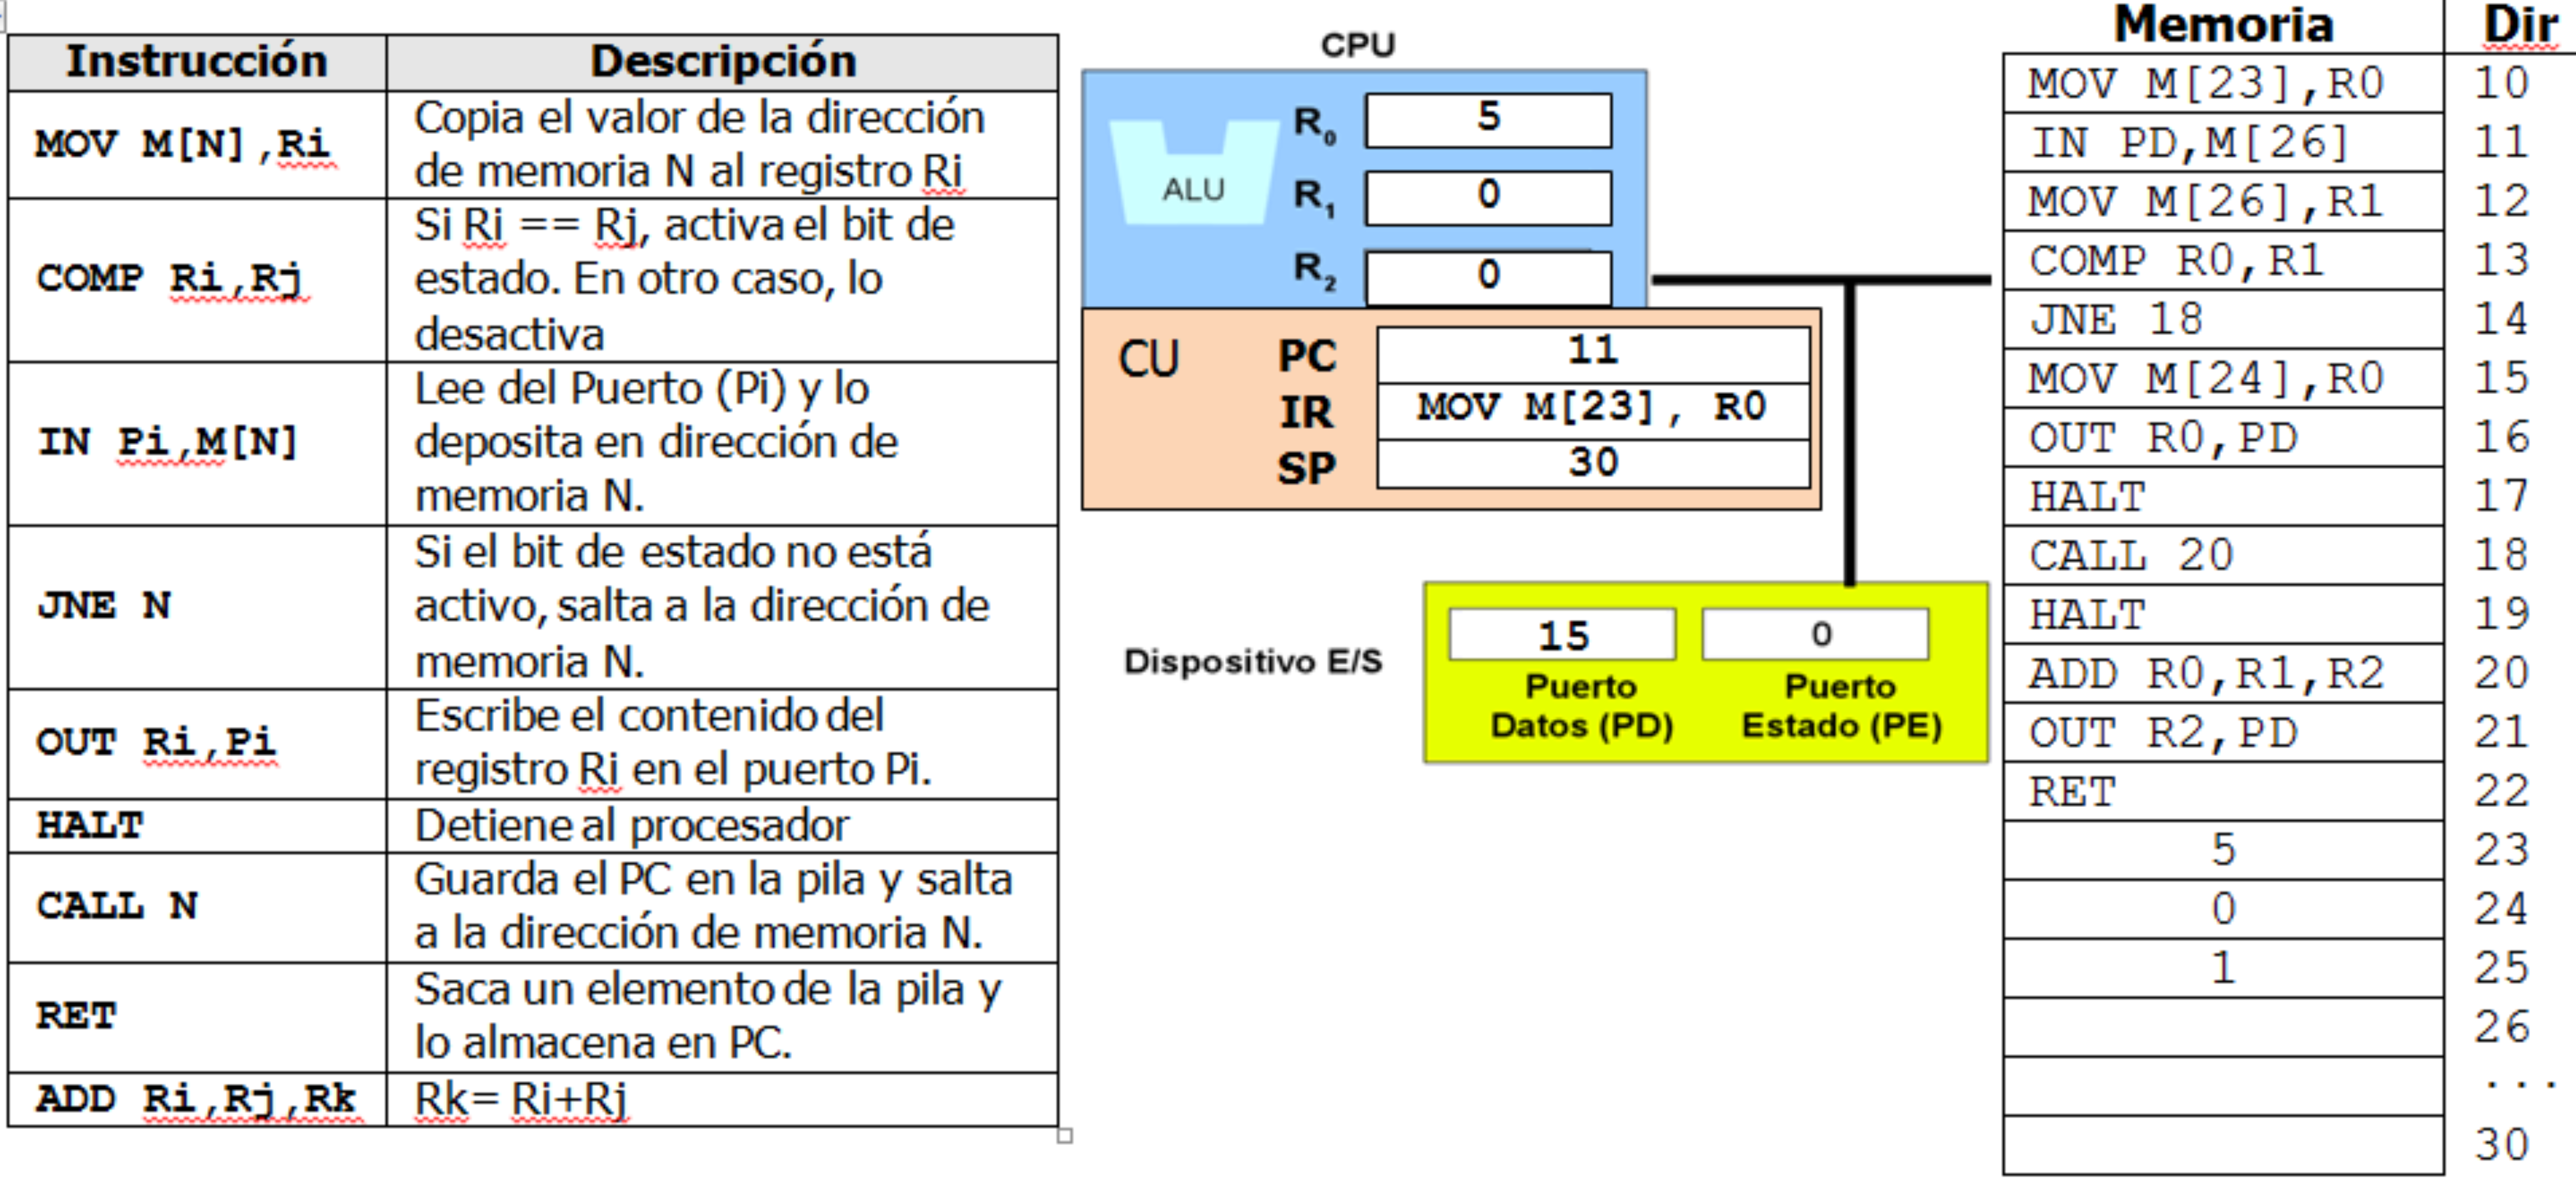
\includegraphics[width=1.1\linewidth]{Imagenes/Ej9_Compuatdor.png}
        \caption{Computador del ejercicio \ref{ej:1.Ejercicio9}}
        \label{fig:Ej9_Computador}
    \end{figure}
    
    El estado del computador en cada ciclo es:
    \begin{table}[H]
        \centering
        \begin{tabular}{c|c|c|c|c|c|c|c}
            PC & IR & SP & R0 & R1 & R2 & PE & PD \\ \hline
            11 & MOV M[23], R0 & 30 & 5 & 0 & 0 & 0 & 15 \\
            12 & IN PD, M[26] & 30 & 5 & 0 & 0 & 0 & 15 \\
            13 & MOV M[26], R1 & 30 & 5 & 15 & 0 & 0 & 15 \\
            14 & COMP R0, R1 & 30 & 5 & 15 & 0 & 0 & 15 \\
            $\cancel{15}$ 18 & JNE 18 & 30 & 5 & 15 & 0 & 0 & 15 \\
            $\cancel{19}$ 20 & CALL 20 & 29 & 5 & 15 & 0 & 0 & 15 \\
            21 & ADD R0, R1, R2 & 29 & 5 & 15 & 20 & 0 & 15 \\
            22 & OUT R2, PD & 29 & 5 & 15 & 20 & 0 & 20 \\
            $\cancel{23}$ 19 & RET & 30 & 5 & 15 & 20 & 0 & 20 \\
            20 & HALT & 30 & 5 & 15 & 20 & 0 & 20
        \end{tabular}
        \caption{Ejecución del programa del ejercicio \ref{ej:1.Ejercicio9}}
        \label{tab:Ejercicio9}
    \end{table}

    \begin{table}[H]
        \centering
        \begin{tabular}{|c|c}
            Memoria & \\ \hline
             & 10 \\
             & $\vdots$ \\
             & 22\\
            5 & 23\\
            0 & 24\\
            1 & 25\\
            15 & 26\\
             & $\vdots$ \\
            19 & 30\\
        \end{tabular}
        \caption{Memoria del ejercicio \ref{ej:1.Ejercicio9}}
        \label{tab:MemEjercicio9}
    \end{table}
\end{ejercicio}
